\chapter{Diseño}
\label{disenio}

\epigraph{La mejor estructura no garantizará los
resultados ni el rendimiento. Pero la
estructura equivocada es una garantía de
fracaso.}%
{\textbf{Peter Drucker}}

\par Según la IEEE el diseño es definido como: \emph{``El proceso de definición de la arquitectura, componentes, interfaces y otras características de un sistema o componente que resulta de este proceso''}[IEEE610.12-90]. Así, todo sistema necesita de un diseño adecuado que permita modelar adecuadamente los requerimientos con el objetivo de tener una mirada integradora del sistema. Un buen diseño ayuda a crear software con propiedades deseables, como reusabilidad, mantenibilidad, portabilidad, ente otras.

\par De manera similar a la elicitación de requerimientos, la descripción detallada del diseño se encuentra documentada en la “Especificación de Diseño de Software”. Análogamente a los capítulos anteriores, sólo se detallarán los aspectos más relevantes del diseño, dejando como lectura adicional el mencionado documento.
 
\section{Responsibility-Driven Design}
\par Este esquema fue empleado para el análisis y descripción del diseño de \textbf{Remo}. Fue propuesto inicialmente por Rebeca Wirfs-Brock y Brian  \\
Wilkerson\cite{ResponsibilityDesign} en 1990. Básicamente, se enfoca en qué responsabilidades deben ser cubiertas por el sistema y en cuáles serán los objetos responsables de llevarlas a cabo. 

\par Inicialmente, se describen las acciones y actividades que constituyen las ``responsabilidades'' del sistema. Luego, se describen dichas responsabilidades en un lenguaje comprensible, tanto para el usuario como para el desarrollador, y finalmente, se diseñan objetos de software que las implementen apropiadamente. En primera instancia, se captura la noción de cuál es el comportamiento deseado, antes de plantear la forma de obtener dicho comportamiento.

\section{Principios de Diseño}
\par Uno de los requerimientos de \remo fue que se respetara los principios del diseño orientado a objetos resumidos en el acrónimo SOLID\cite{Martin00} introducido por Robert C. Martin\footnote{Autor de varios libros tales como ``Object-orineted Design'' y ``Agile Development''.} a principios del año 2000.

\par En particular se puso especial atención en respetar los principios SRP, OCP y DIP debido a que repercuten directamente en que el sistema sea más simple de mantener y extender con nuevas funcionalidades. Además, el principio DIP es fundamental para lograr un software que sea verificable mediante la automatización de pruebas como se pudo comprobar más adelante, en la etapa de “verificación”.

A continuación se detalla brevemente cada uno de los principios, dado que resultan de gran importancia su conocimiento.

\begin{itemize}
	\item \textbf{Principio de Simple Responsabilidad (SRP):} establece que no debería haber nunca más de una sola razón para que una clase cambie. En el contexto de este principio, llamamos responsabilidad a una razón de cambio. Si una clase tiene más de una responsabilidad, las responsabilidades se acoplan. Esta clase de acoplamiento lleva a que el sistema no sea tolerante a las modificaciones. Básicamente, refiere a la noción de que un objeto debe tener sólo una responsabilidad.
	
	\item \textbf{Principio de Apertura-Cierre (OCP):} este principio afirma que las entidades de software (clases, módulos, funciones, etcétera) deben estar abiertas para la extensión, pero cerradas para la modificación. Esto es especialmente valioso en un entorno de producción, donde los cambios en el código fuente puede requerir revisiones de código, pruebas unitarias, y otros procedimientos para calificar para su uso en un producto.
	\par Este principio indica que cuando se cambian los requisitos, se extiende el comportamiento de los módulos mediante la adición de código, pero el código viejo no se cambia dado que funciona.

	\item \textbf{Principio de Sustitución de Liskov (LSP):} refiere a que los objetos de un programa pueden ser reemplazados por instancias de sus subtipos, sin alterar la exactitud del programa.
	\par Se afirma que, en un programa, si \textsc{S} es un subtipo de \textsc{T} (\textsc{T}$\to$\textsc{S}), entonces los objetos de tipo \textsc{T} puede ser reemplazado con los objetos de tipo \textsc{S} sin alterar ninguna de las propiedades deseables de ese programa. Más formalmente, el principio LSP es una definición particular de una relación de subtipificación, que fue introducido inicialmente por Bárbara Liskov\cite{liskov}. Se trata de una relación semántica más que sintáctica que tiene la intención de garantizar la interoperabilidad semántica de los tipos en una jerarquía, los tipos de objeto en particular. 

	\item \textbf{Principio de Segregación de Interfaz (ISP):} refiere a la idea de que varias interfaces específicas son mejores que una interface de uso general.
	\par Es un principio utilizado para un desarrollo limpio. Si se cumple, ayuda a mantener un sistema desacoplado y por lo tanto más fácil de refactorizar. El ISP dice que una vez que una interfaz se ha vuelto demasiado ``gorda'' debe ser dividida en interfaces más pequeñas y más específicas para que los clientes sólo tengan disponibles los métodos que pertenecen a ellos. En pocas palabras, los clientes no deberían ser obligados a depender de interfaces que no usan. 

	\item \textbf{Principio de Inversión de Dependencia (DIP):} refiere al sentido en que se debe depender de las abstracciones y no de las concreciones.
	\par Los módulos de alto nivel no deben depender de módulos de bajo nivel y ambos deberían depender de las abstracciones. Además establece que las abstracciones no deben depender de los detalles. Los detalles deberían depender de las abstracciones. 
\end{itemize}

\section{Arquitectura del Sistema}
\par Según \cite{arquitecturaSistema} ``la \emph{arquitectura} es un nivel de diseño que hace foco en aspectos más allá de los algoritmos y estructuras de datos de la computación; el diseño y especificación de la estructura global del sistema es un nuevo tipo de problema''.

\par \remo está compuesto por 4 componentes básicos como se observar en la figura~\ref{componentesBasicos}:

\begin{enumerate}
	\item Generador de secuencias humanizadas: encargado de humanizar secuencias, es decir, cambiar los codones según el organismo especificado.

	\item Generador de análisis de secuencias: tiene como tarea realizar el análisis entre las secuencias de $_m$RNA vs. $_m$$_i$RNA.

	\item Generador de comparaciones de estructuras: encargado de la comparación entre estructuras secundarias, para lo cual necesita de el reconocimiento de motifs.

	\item PreFold: encargado de realizer el folding de secuencias.

\end{enumerate}

\begin{figure}[!hbtp]
	\begin{center}
		\hspace*{.6cm}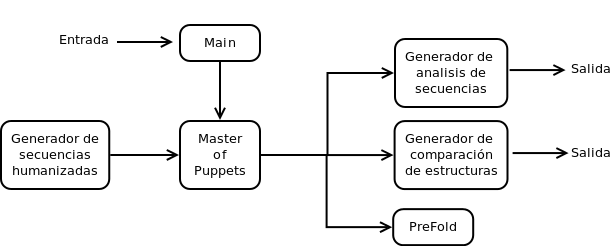
\includegraphics[width=12.5cm, height=5.2cm]{image/componenteRemo.png}
		\caption{Componentes de \textbf{Remo} [2].}
		\label{componentesBasicos}
	\end{center}
\end{figure}

\par En la figura~\ref{arquitecture} se exhibe con más detalle el diseño arquitectónico de \textbf{Remo}.

% \newpage
\begin{figure}[!hbtp]
	\begin{center}
		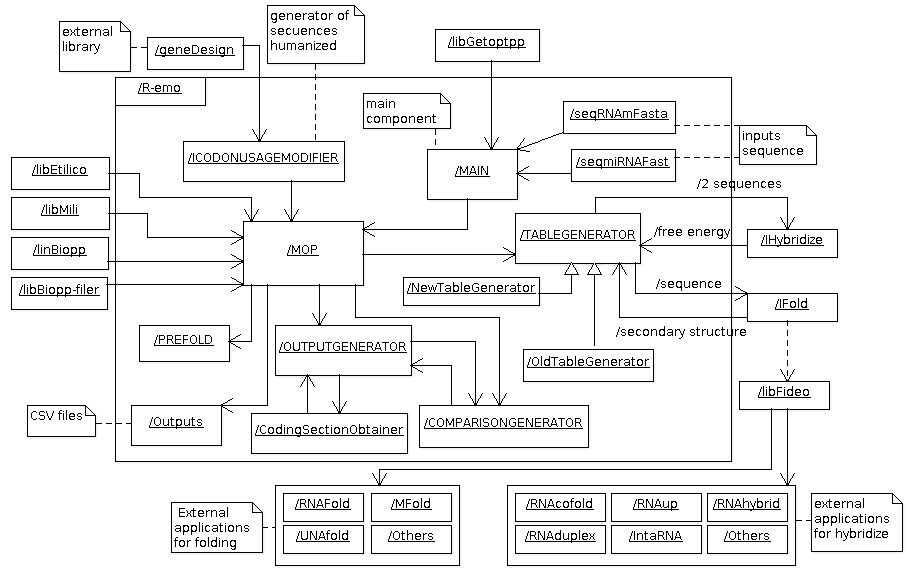
\includegraphics[width=20cm, height=12cm, angle=90]{image/arquitectura.png}
		\caption{UML - Arquitectura del Sistema [2]} 
		\label{arquitecture}
	\end{center}
\end{figure}

\subsection{Catálogo de componentes}
\par A continuación se especifican los distinto componentes de \textbf{Remo}:

\begin{itemize}
	\item \textbf{Main:} punto de entrada de \textbf{Remo}.
	\item \textbf{MOP:} mediador responsable de la comunicación entre los módulos del sistema.

	\item \textbf{CodingSectionObtainer:} permite obtener la mayor sección codificante de una secuencia.

	\item \textbf{TableGenerator:} interfaz para seleccionar el tipo de salida de \textbf{Remo}.

	\item \textbf{OldTableGenerator:} emplea un método ad-hoc usando los backend de folding.

	\item \textbf{NewTableGenerator:} emplea un método formal empleando los backends de hidridacíon.

	\item \textbf{OutputGenerator:} permite obtener los archivos de resultado.

	\item \textbf{ComparisonGenerator:} permite realizar la comparación de estructuras secundarias (parser).

	\item \textbf{Prefold:} permite realizar el folding de las secuencias de $_m$RNA. 
\end{itemize}

\subsection{Comportamiento Dinámico}
En la figura~\ref{compDinamico} se expone un diagrama de secuencia que permite visualizar la interacción dinámica entre los componentes de \remo para el análisis de secuencias de $_m$RNA y $_m$$_i$RNA.

\begin{figure}[!hbtp]
	\begin{center}
		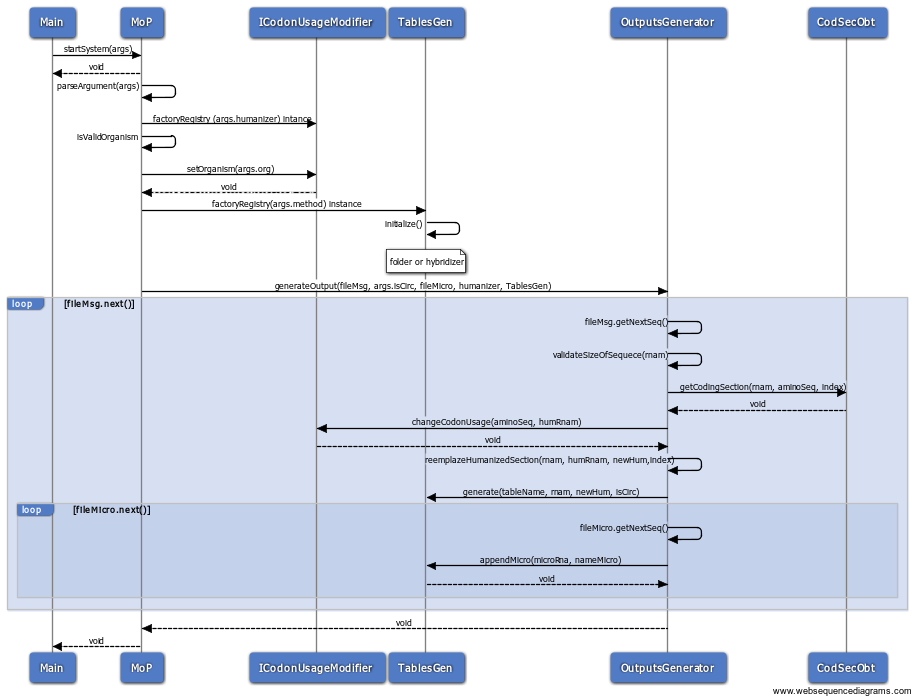
\includegraphics[width=20cm, height=16cm, angle=90]{image/remoCompDin.png}
		\caption{Interacción dinámica entre los componentes de \textbf{Remo} [2].}
		\label{compDinamico}
	\end{center}
\end{figure}

\section{Diseño de Medio Nivel}
\subsection{Diagrama de Paquetes}
\par En la figura~\ref{paquetesDiag} se exhiben el diagrama de paquetes correspondiente a \textbf{Remo}, donde se exhiben las distintas librerías que interactúan.

\begin{figure}[!hbtp]
	\begin{center}
		\vskip 1cm
		\hspace*{1cm}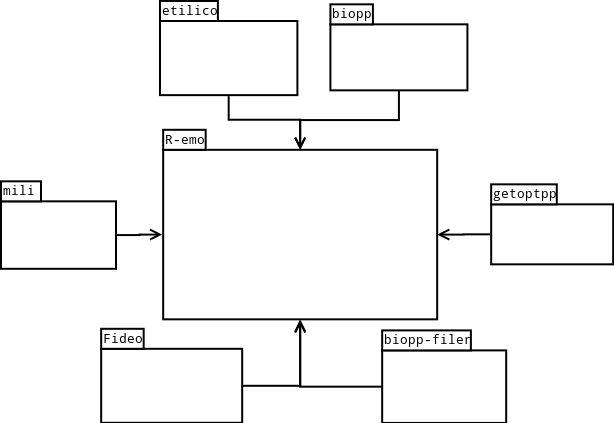
\includegraphics[width=13.5cm, height=10cm]{image/packageDiagramHighGranularity.png}
		\caption{UML - Diagrama de Paquetes [2].}
		\label{paquetesDiag}
	\end{center}
\end{figure}

\subsection{Diagrama de Clases}
\par En la figura~\ref{RemoDClase1} se exhibe un diagrama de clases de \textbf{Remo}. Con el objetivo de lograr una mejor comprensión, se decidió no especificar los métodos y miembros de cada clases. Para mayor detalle puede visitar el apéndice~\ref{disenioEnDetalles} (figuras ~\ref{remoDClase1} y ~\ref{remoDClase2}).

\begin{figure}[!hbtp]
	\begin{center}
		\hspace*{-1.5cm}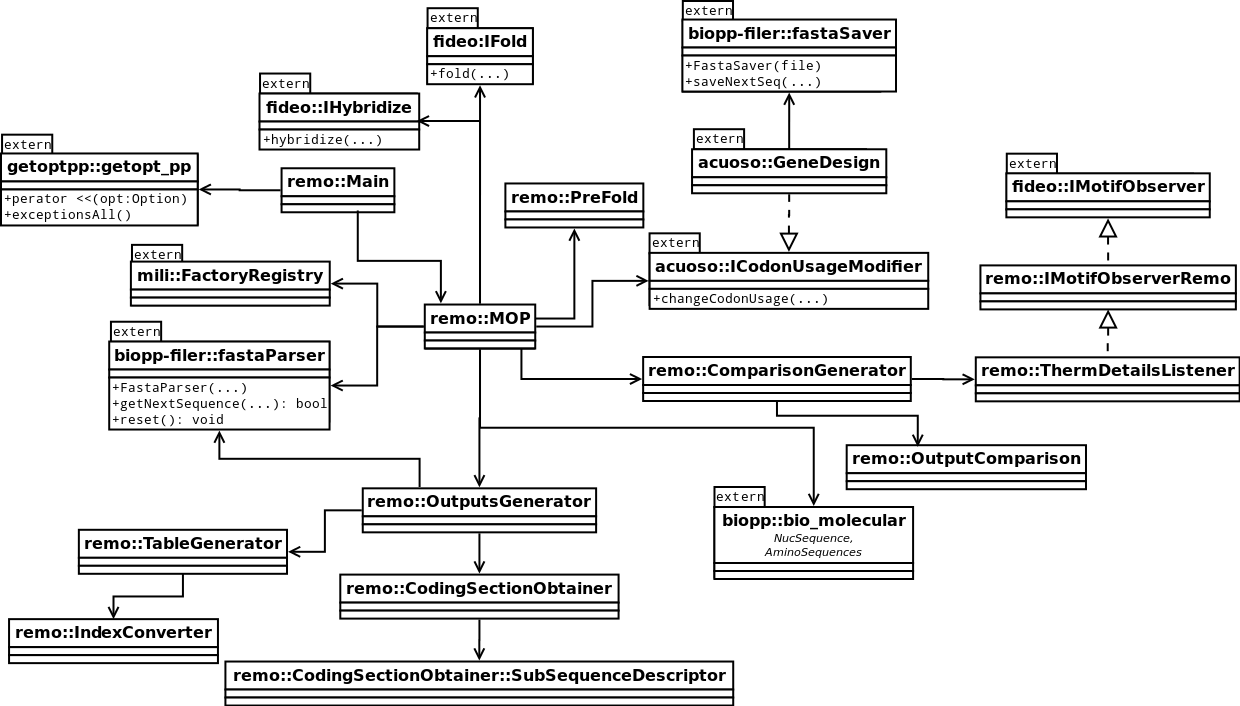
\includegraphics[width=19cm, height=12.5cm, angle=90]{image/emptyClass.png}
		\caption{UML - Diagrama de clases de \textbf{Remo} [2].}
		\label{RemoDClase1}
	\end{center}
\end{figure}

\vskip 15cm
\section{Nuevas Librerías}
\subsection{Fideo: Folding Interface Dynamic Exchange Operations}

\par Tal como se mencionó en la sección~\ref{libreriaAImplementar}, fideo proveerá los servicios necesarios para folding e hibridación. Para tal fin, se empleó el patrón de diseño \emph{Factory Method}(ver Apéndice~\ref{factoryMethod}). Por otra parte, fideo proporciona un parser para identificar motifs en estructuras secundarias. Para tal fin se empleó el patrón de diseño \emph{Observer}(ver Apéndice~\ref{observer}). Para implementar el método \emph{fold()} propiamente dicho se empleó el patrón de diseño \emph{Template Method}(ver Apéndice~\ref{templateMethod}).

En la figura~\ref{interfaceFideo} se exhiben las interfaces implementadas con sus respectivas clases concretas. Se puede observar la interfaz \emph{IMotifObserver} y \emph{IRule} no mencionadas hasta el momento. Básicamente se busca emplear un observer, esto es, fideo proporcionará el parser de estructuras secundarias y establecerá una interfaz la cual deberá ser implementada por \remo para realizar en correspondiente análisis.

\par En este contexto, se puede apreciar la idea del principio de diseño \emph{DIP}. Dado que, si \remo depende de estas interfaces y no de sus respectivas implementaciones se consigue abstraer los detalles de cada librería externa y lograr un software mas versátil. 

\begin{figure}[!hbtp]
	\begin{center}
		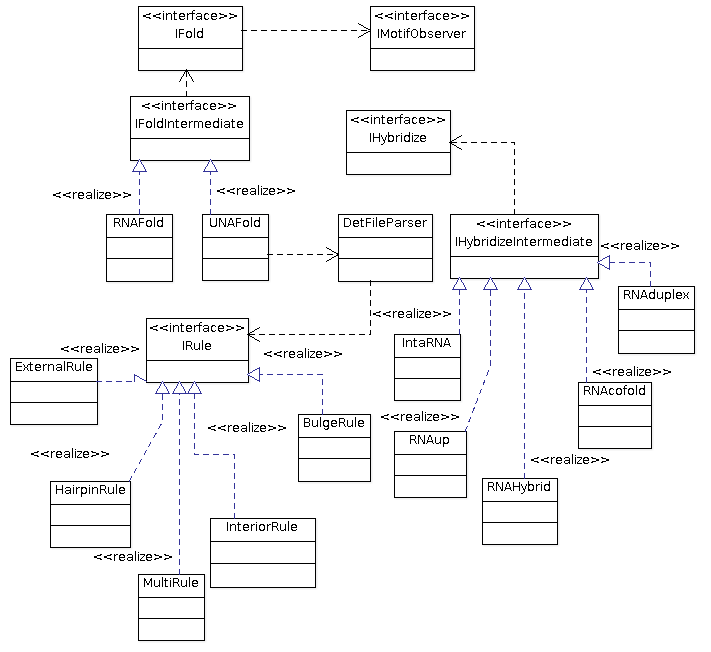
\includegraphics[width=15cm, height=13.5cm]{image/fideoInterface.png}
		\caption{UML - Interfaces de fideo. [2]}
		\label{interfaceFideo} 
	\end{center}
\end{figure}

\par El diagrama de clases correspondiente a fideo puede observarse en la figura~\ref{fideitoDisenio1}. Al igual que en \remo, para lograr una mejor comprensión, se decidió no especificar los métodos y miembros de cada clases, puede visitar el apéndice~\ref{disenioEnDetalles} (figuras~\ref{fideoDisenio1} y ~\ref{fideoDisenio2})para mayor detalle.

\begin{figure}[!hbtp]
	\begin{center}
		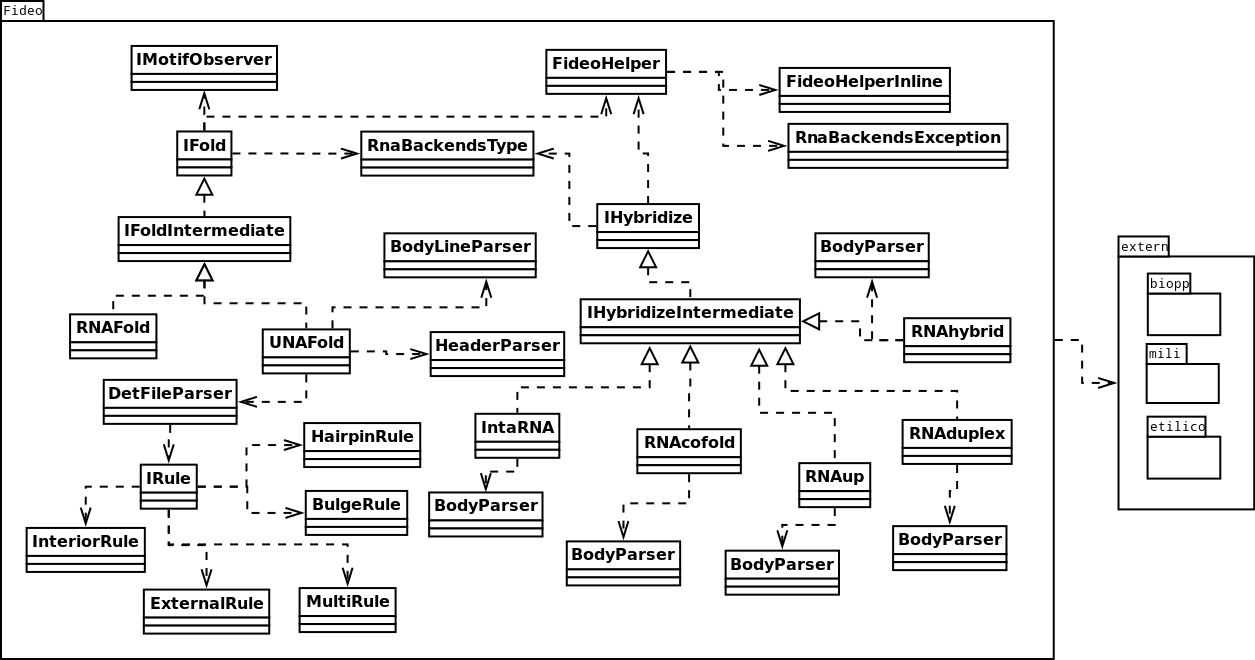
\includegraphics[width=20.5cm, height=13cm, angle=90]{image/clasesFideo.png}
		\caption{UML - Diagrama de clases de fideo [2].}
		\label{fideitoDisenio1}
	\end{center}
\end{figure}

\vskip 10cm
\subsection{Acuoso: Abstract Codon Usage Optimization Software for Organisms}
Esta librería sigue la misma idea de fideo, se definió una interfaz \emph{ICodonUsafeModifier} de modo que sea transparente el uso de cualquier software o método de humanización. En la figura~\ref{acuosoInterface} se observa el diagrama de clases correspondiente.

\begin{figure}[!hbtp]
	\begin{center}
		
\includegraphics[width=15.5cm, height=7.5cm]{image/acuoso.png}
		\caption{UML - Diagrama de clases de Acuoso [2].}
		\label{acuosoInterface}
	\end{center}
\end{figure}

\subsection{Etilico: External Tools Invocation LIbrary COmponent}
\par Etilico corresponde a una librería estática contenedora de diversos métodos necesarios cuyo diseño es muy simple. En la figura~\ref{disenioEtilico} se exhibe el diagrama las clases contenidas en etilico.
\par La clase \emph{Helper} contiene diferentes funciones de gran utilidad. La clase \emph{TmpDirectory}, representa el manejo de directorios temporales, y por último, la clase \emph{Config} se trata de un singletón (ver Apéndice~\ref{singleton}) empleado para configurar las diferentes rutas de las herramientas empleadas.

\begin{figure}[!hbtp]
	\begin{center}
		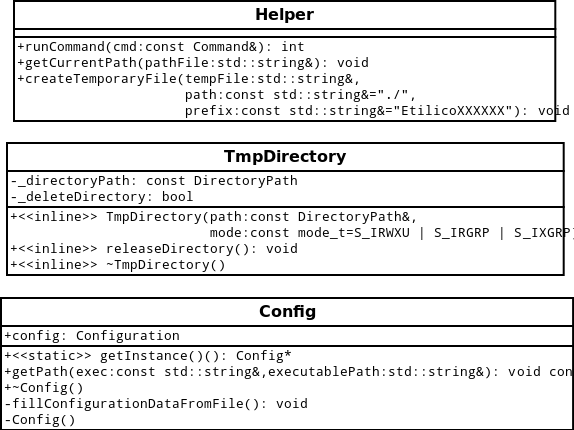
\includegraphics[width=13cm, height=8.5cm]{image/etilico.png}
		\caption{UML - Diagrama de clases de etilico [2].}
		\label{disenioEtilico}
	\end{center}
\end{figure}